\setcounter{chapter}{8}
\setcounter{section}{4}
\setcounter{question}{0}

%%%%%%%%%%%%%%%%%%%%%%%%%%%%%%%%%%%%%%%%%%%%%%%%%%%%%%%%%%%%%%%%%%%%%%%%%%%
% Assignment 8.4: Comparing simple models using the Bayes factor
%%%%%%%%%%%%%%%%%%%%%%%%%%%%%%%%%%%%%%%%%%%%%%%%%%%%%%%%%%%%%%%%%%%%%%%%%%%

\rassignment{Comparing simple models using the Bayes factor}

Bayesian statistics does not use the \concept{p-value} to test hypotheses and yield conclusions in an all-or-none fashion. Instead it uses a continuous measure of evidence, the \concept{Bayes factor}. The \concept{Bayes factor} quantifies the relative predictive performance of two competing hypotheses; the \concept{null hypothesis} $H_0$ and the \concept{alternative hypothesis} $H_1$. The subscript in the \concept{Bayes factor} indicates for which hypothesis support is quantified. $BF_{10}$ indicates the Bayes factor in favor of $H_1$ over $H_0$, whereas $BF_{01}$ indicates the \concept{Bayes factor} in favor of $H_0$ over $H_1$. Larger values of $BF_{10}$ indicate more support for $H_1$. A \concept{Bayes factor} can range from 0 to $\infty$, and a Bayes factor of 1 indicates that both hypotheses are supported equally well by the data. A $BF_{10} = 10$ indicates that the data is 10 times more likely to occur under $H_1$ than under $H_0$. Given this interpretation, the \concept{Bayes factor} is a continuous measure for the strength of evidence. \\

Suppose you are a data scientist at a stock trading company. You have written an algorithm that trades stocks automatically. Your algorithm either makes a profitable trade, or a losing trade. You want to make sure that your algorithm actually does something intellectual, and therefore want to disprove the hypothesis that your algorithm makes a profitable trade with a probability other than if it were to trade stocks randomly. \\

\question{Specify the \concept{null hypothesis} $H_0$ and the \concept{alternative hypothesis} $H_1$ for the test of a proportion $\theta$ against a chance value.}

\hypothesesbox

\question{Specify a $Beta$ prior distribution for the \concept{parameter} $\theta$. Let your prior distribution depend on how much confidence you have in your programming skills.}

\hint{Think about what the $\theta$ represents in this case.}

\emptyanswerbox{
\begin{center}
    $\theta \sim Beta($\tinyanswerline, \tinyanswerline)
\end{center}
}

You monitor the algorithm for 30 trades, and each time mark a trade as a success (profit) or a failure (loss). After data collection you see that, of the 30 trades, your algorithm made 22 profitable trades. \\

\question{
    What are the $\alpha$ and $\beta$ parameters of your \concept{posterior distribution}?
}

\emptyanswerbox{
    $\alpha$: \shortanswerline \hspace*{3cm} $\beta$: \shortanswerline
}

\clearpage % Page break

\question{Use the \rcode{curve()} function to create a figure showing both the prior and the posterior distribution.}

\hint{The \rcode{curve()} function has an argument \rcode{add} that controls whether to add a line to an already existing plot.}

\rcodeanswertiny

In this scenario, the \concept{Bayes factor} is intuitively to calculate by only looking at the posterior distribution for $H_1$. The \concept{Bayes factor} $BF_{10}$ tells you how much more likely the \concept{alternative hypothesis} $H_1$ is in comparison with to the point \concept{null hypothesis} $H_0$. The \concept{Bayes factor} $BF_{10}$ in favor of the unrestricted \concept{alternative hypothesis} $H_1: \theta \neq 0.5$ is simply the height of the \concept{posterior distribution} at the point $\theta = 0.5$ divided by the height of the \concept{prior distribution} at the point $\theta = 0.5$. \\

Please note that this is a trick that only works for \concept{nested} hypotheses and models, in which only one of the \concept{parameters} is fixed to a specific value. \\

\begin{center}
    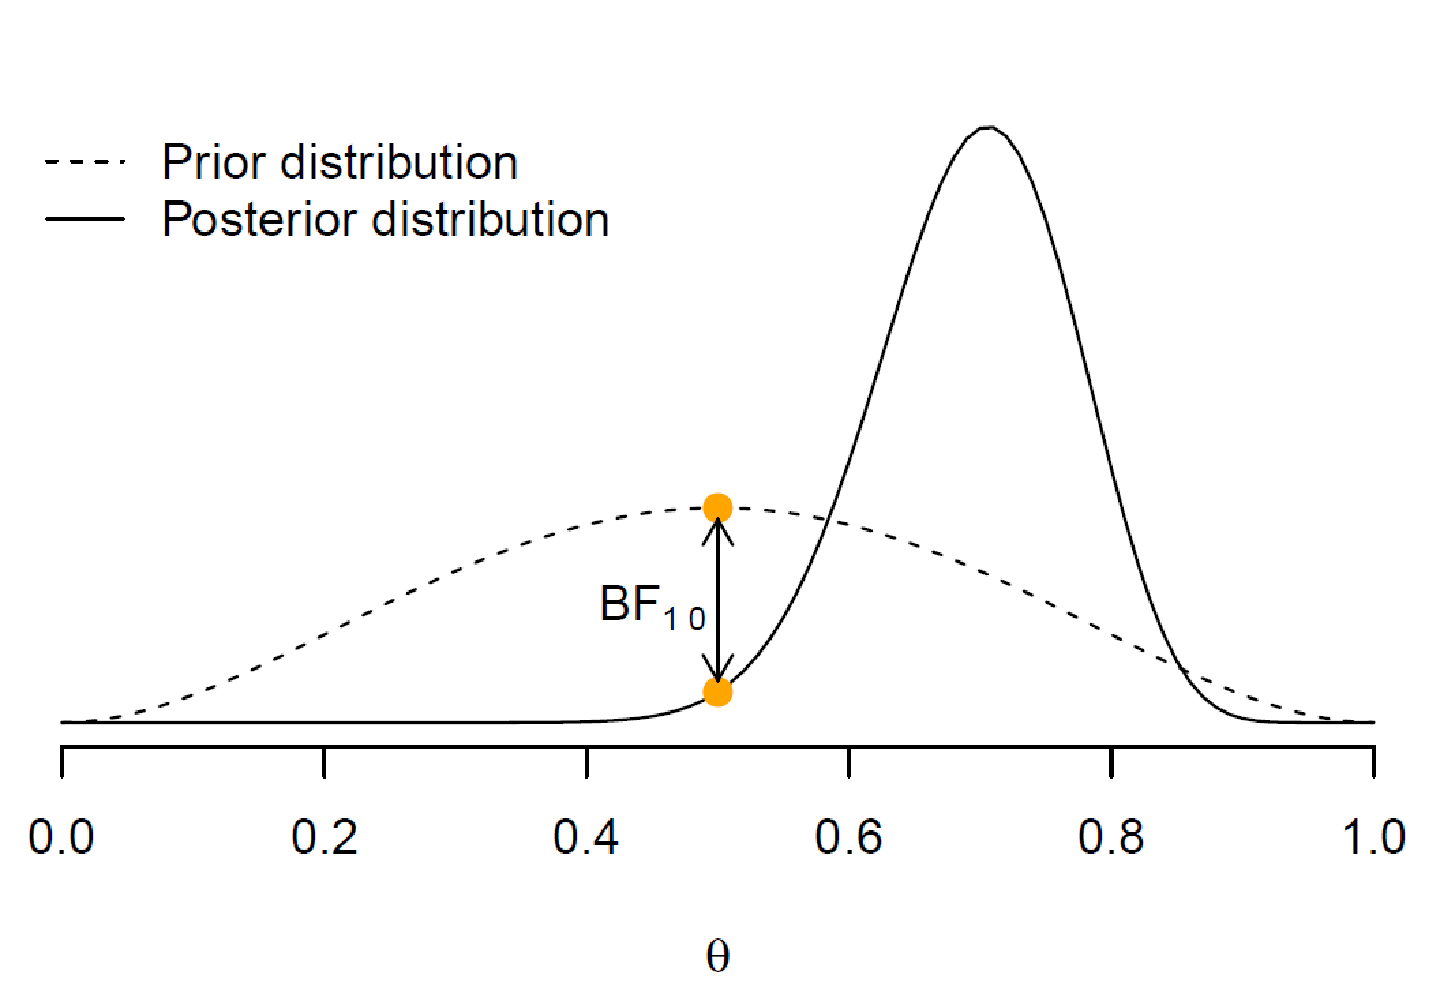
\includegraphics[width=0.6\textwidth]{Files/Images/priorAndPosterior.pdf}
\end{center}

\question{Use the \rcode{dbeta()} function to find out the height of your \concept{prior distribution} at the point $\theta = 0.5$ and store it in an object called \rcode{heightPrior}.}

\rcodeanswertiny

\question{Use the \rcode{dbeta()} function to find out the height of your \concept{posterior distribution} at the point $\theta = 0.5$ and store it in an object called \rcode{heightPosterior}.}

\rcodeanswertiny

\clearpage % Page break

Run the following code in \texttt{R} to compute the \concept{Bayes factor} in favor of the \concept{alternative hypothesis} $H_1$. \\
\\
\codeblock{BF10 <- heightPrior / heightPosterior}

\question{What is the value of the \concept{Bayes factor} \rcode{BF10}? Interpret this \concept{Bayes factor} with respect to the alternative hypothesis $H_1$.}

\twolineanswerbox

To make interpretation of the \concept{Bayes factor} more simple, the labels in the table below have been proposed. Please note that you shout not get too hung up on the specific labels and breakpoints in this table, since what constitutes convincing evidence should be different in every situation. \\

\begin{table}[h]
    \centering
    \begin{tabular}{r|l}
         Bayes factor & Evidence \\
         \hline
         1 - 3 & Anecdotal \\
         3 - 10 & Moderate \\
         10 - 30 & Strong \\ 
         30 - 100 & Very strong \\
         $>$ 100 & Extreme
    \end{tabular}
\end{table}

\question{Considering the labels from the table above, are you convinced enough to reject the hypothesis that your algorithm makes a profitable trade with a probability other than if it were to trade stocks randomly?}

\twolineanswerbox

\question{Re-specify the $\alpha$ and $\beta$ parameters of the \concept{prior distribution} so that you express a different prior belief. Recalculate the \concept{Bayes factor} by running your code again. What is the new value of \rcode{BF10}. How robust in your \concept{Bayes factor} to changes in the prior distribution?}

\onelineanswerbox

\clearpage % Page break